\documentclass[dvipdfmx, fleqn]{jsarticle}
\usepackage{geometry}
\usepackage{multicol}
\usepackage{ascmac}
\usepackage{emathPh}
\usepackage{amsmath}
\usepackage{color}
\geometry{top=20mm, bottom=20mm, left=15mm, right=15mm}
\renewcommand{\baselinestretch}{1.3}
\newcount\ansFlag
\ansFlag=0

\newcommand{\ans}[1]{
\ifnum\ansFlag=0
\phkasen<kasenUehosei=0.5em>{
\hspace{0.5em}\textcolor{white}{#1}
\hspace{0.5em}
}
\else
\phkasen<kasenUehosei=0.5em>{
\hspace{0.5em}\textcolor{red}{#1}
\hspace{0.5em}
}
\fi
}

\newcommand{\nyquistAns}{
\ifnum\ansFlag=0
\begin{figure}[ht]
	\hspace{5em}
	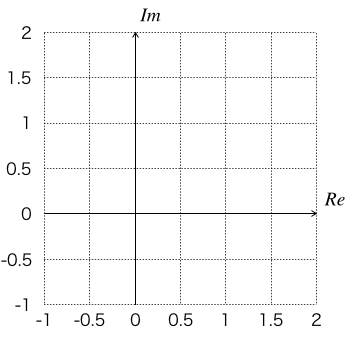
\includegraphics[height=65mm]{figure/nyquistQues.png}
\end{figure}
\else
\begin{figure}[ht]
	\hspace{5em}
	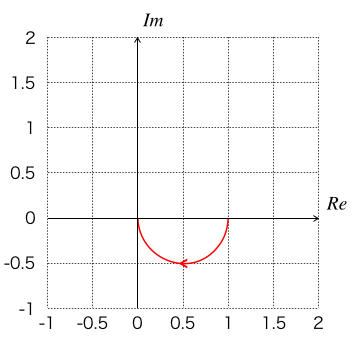
\includegraphics[height=65mm]{figure/nyquistAns.png}
\end{figure}
\fi
}

\begin{document}
\renewcommand{\labelenumi}{(\arabic{enumi})}
\begin{itembox}[l]{\textbf{問題}}
	\hspace{1em}伝達関数が
	\vspace{0.8em}
	\[
	G(s) = \frac2{s + 2}
	\]
	で与えられる1次遅れ要素について以下の問いに答えよ.
	\begin{enumerate}
		\item ステップ応答を求めよ.
		\item ナイキスト線図の概形を描け.
		\item ボード線図の概形を描け.($但し, \log_2 = 0.30とする.$)
	\end{enumerate}
\end{itembox}

\begin{enumerate}
	\item ステップ応答を求めよ. \\
	ステップ関数$u(t)$をラプラス変換すると, \\
	ラプラス変換表より $U(s) = \mathcal{L}[u(t)] = \ans{\dfrac 1s}$ \\
	$Y(s) = G(s)\cdot U(s) = \dfrac2{s + 2}\cdot{\dfrac 1s}$ \\
	この式を部分分数分解すると,
	\mathindent = 0mm
	\begin{multicols}{2}
		\noindent
		\begin{align*}
			\dfrac2{s + 2}\cdot{\dfrac 1s} &= \ans{\dfrac a{s + 2} + \dfrac bs} \\
			&= \dfrac {as + b(s + 2)}{s(s + 2)} \\
			&= \dfrac {(a + b)s + 2b}{s(s + 2)}
		\end{align*}
		\columnbreak
		\(
		\ans{
		\begin{cases}
			a + b = 0 \\
			2b = 2
		\end{cases}
		}
		\Rightarrow
		\begin{cases}
			a  = -1 \\
			b = 1
		\end{cases}
		\)
	\end{multicols}
	 $∴ Y(s) = \ans{-\dfrac 1{s + 2} + \dfrac1s}$ \\
これをラプラス逆変換してステップ応答を求めると, \\
ラプラス変換表より $y(t) = \mathcal{L}^{-1}\left[-\dfrac 1{s + 2} + \dfrac1s\right] = \ans{-e^{-2t} + 1 = 1 - e^{-2t}}$

\vspace{3em}
	\item ナイキスト線図の概形を描け. \\
	この伝達関数の周波数応答は, $G(j\omega) = \ans{\dfrac2{j\omega + 2}}$ \\
	これを変形すると,
	\noindent
	\begin{align*}
		G(j\omega) &= \dfrac2{j\omega + 2} \\
		&= \ans{\dfrac{2(2 -j\omega)}{(2 + j\omega)(2 - j\omega)}} \\
		&= \dfrac{4 - 2j\omega}{4 + \omega^2} \\
		&= \ans{\dfrac 4{4 + \omega^2} - \dfrac {2\omega}{4 + \omega^2}j}
	\end{align*}
	\newpage
		実部, 虚部をそれぞれ$x, y$と置くと, \\
		\(
		\begin{cases}
			x = Re(G(j\omega)) = \ans{\dfrac4{4 + \omega^2}} \\
			y = Im(G(j\omega)) = \ans{-\dfrac{2\omega}{4 + \omega^2}}
		\end{cases}
		\)
		\begin{multicols}{3}
			\noindent
		\begin{align*}
			&x = \dfrac4{4 + \omega^2} \\
			&\to (4 + \omega^2)x = 4 \\
			&\to \omega^2x = 4 - 4x \\
			&\to \omega^2 = \dfrac{4(1-x)}x \\
			&\to \omega = 2\sqrt{\dfrac{1-x}x}
		\end{align*}

		\columnbreak

		\noindent
		\begin{align*}
			y &= - \dfrac{2\cdot2\sqrt{\dfrac{1-x}{x}}}{4 + 4\left(\dfrac{1-x}x\right)} \\
			&= -\dfrac{4\sqrt{\dfrac{1-x}{x}}}{4\left( 1 + \dfrac{1-x}x\right)} \\
			&= -\dfrac {\sqrt{\dfrac {1-x}x}}{\dfrac{x + 1 - x}x} \\
			&= -\dfrac {\sqrt{\dfrac {1-x}x}}{\dfrac 1x} \\
			&= -x\sqrt{\dfrac {1-x}x} \\
			&= -\sqrt{x^2\cdot\dfrac {1-x}x} \\
			&= -\sqrt{x(1-x)} \\
		\end{align*}

		\columnbreak

		\noindent
		\begin{align*}
			&y^2 = x(1-x) \\
			&\to y^2 = x - x^2 \\
			&\to y^2 = -(x^2 - x) \\
			&\to y^2 = - \left\{x^2 - 2\cdot\dfrac12x + \left(\dfrac12\right)^2\right\} + \left(\dfrac12\right)^2 \\
			&\to y^2 = - \left(x - \dfrac12\right)^2 + \left(\dfrac12\right)^2 \\
			&\to \ans{\left(x - \dfrac12\right)^2 + y^2 =  \left(\dfrac12\right)^2}
		\end{align*}
	\end{multicols}
	よって, $中心\ans{(0.5,\ 0)}, 半径\ans{0.5}を通る円を描くことが分かる.$ \\
	但し, $0<\omega<\infty$のとき, $\ans{y<0}$であることから,$y<0$の範囲のみを通る半円であることが分かる. \\
	また,ナイキスト線図の方向を確認すると, \\
	$\displaystyle\lim_{\omega\to0}x = \displaystyle\lim_{\omega\to0}\dfrac4{4 + \omega^2} = \dfrac4{4 + 0^2} = 1$ \\
	$\displaystyle\lim_{\omega\to\infty}x = \displaystyle\lim_{\omega\to\infty}\dfrac4{4 + \omega^2} = \dfrac4{4 + \infty^2} = 0$ \\
	よって, ナイキスト線図の概形は以下のようになることが分かる.
	\nyquistAns


	\newpage
	\item ボード線図の概形を描け.($但し, \log_2 = 0.3とする.$) \\
	周波数伝達関数の大きさを求めると,
	\begin{align*}
		|G(j\omega)| &= \ans{\sqrt{\left(\dfrac 4{4 + \omega^2}\right)^2 + \left( - \dfrac {2\omega}{4 + \omega^2} \right)^2}} \\
		&= \sqrt{\dfrac {16}{(4 + \omega^2)^2} + \dfrac {4\omega^2}{(4 + \omega^2)^2}} \\
		&= \sqrt{\dfrac {4(4 + \omega^2)}{(4 + \omega^2)^2}} \\
		&= \dfrac2{\sqrt{4 + \omega^2}}
	\end{align*}
	\begin{multicols}{2}
		よって, ゲインは
		\begin{align*}
			g_{dB} &= \ans{20\log|G(j\omega)|} \\
			&= 20\log\left(\dfrac2{\sqrt{4 + \omega^2}}\right) \\
			&= 20\log2 - 20\log(4 + \omega^2)^{\frac12} \\
			&= 20\cdot0.3 - 10\log(4 + \omega^2) \\
			&= 6 - 10\log(4 + \omega^2)
		\end{align*}

		\columnbreak

		また, 位相は
	\begin{align*}
		\phi(\omega) &= \ans{\tan^{-1}\left(\dfrac{-\dfrac{2\omega}{4 + \omega^2}}{\dfrac4{4 + \omega^2}}\right)} \\
		&=\tan^{-1}\left(\dfrac{-\omega}2\right)
	\end{align*}
\end{multicols} \hspace{1em}

\begin{multicols}{3}
	$\omega = 0のとき,$
	\noindent
	\begin{align*}
		\phi(\omega) &= \tan^{-1}\left(\dfrac02\right) \\
		&= \tan^{-1}0 = 0
	\end{align*}

	\noindent
	\begin{align*}
		g_{dB} &= 6 - 10\log(4 + 0) \\
		&= 6 - 20\log2 \\
		&= 6 - 20\cdot0.3 \\
		&= 6 - 6 = 0
	\end{align*}

	\columnbreak

	$\omega = 2のとき,$
	\noindent
	\begin{align*}
		\phi(\omega) &= \tan^{-1}\left(\dfrac{-2}2\right) \\
		&= \tan^{-1}(-1) = -\dfrac\pi4
	\end{align*}

	\noindent
	\begin{align*}
		g_{dB} &= 6 - 10\log(4 + 4) \\
		&= 6 - 30\log2 \\
		&= 6 - 30\cdot0.3 \\
		&= 6 - 9 = -3
	\end{align*}

	\columnbreak

	$\omega \to \infty のとき,$
	\noindent
	\begin{align*}
		\phi(\omega) &= \lim_{\omega\to\infty}\tan^{-1}\left(\dfrac\omega2\right) =\frac\pi2
	\end{align*}

	\noindent
	\begin{align*}
		g_{dB} &= 6 - \lim_{\omega\to\infty}10\log(4 + \omega^2) \\
		&= 6 - \infty = -\infty
	\end{align*}
\end{multicols}
よって, これらをプロットすると教科書のようなグラフになる.\\
\begin{figure}[ht]
	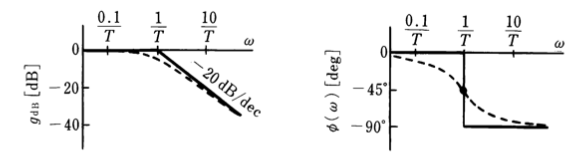
\includegraphics[width=0.8\hsize]{figure/Board.png}
\end{figure}

\end{enumerate}
\end{document}
